\section{\textsc{Rührei auf Vollkornbrötchen}}

\subsection*{Zutaten für 2 Portionen:}

\begin{tabular}{p{7.5cm} p{7.5cm}}
	& \\
	5 Eier & 2 Vollkornbrötchen \\
	1 Tomate & 20g Butter \\
  1EL Kresse & 2 Salatblätter \\
  Frische Käuter & Remoulade \\
  Öl zum Braten & Schluck Mineralwasser \\
  Salz, Pfeffer \& Muskatnuss
\end{tabular}

\subsection*{Serviervorschlag:}

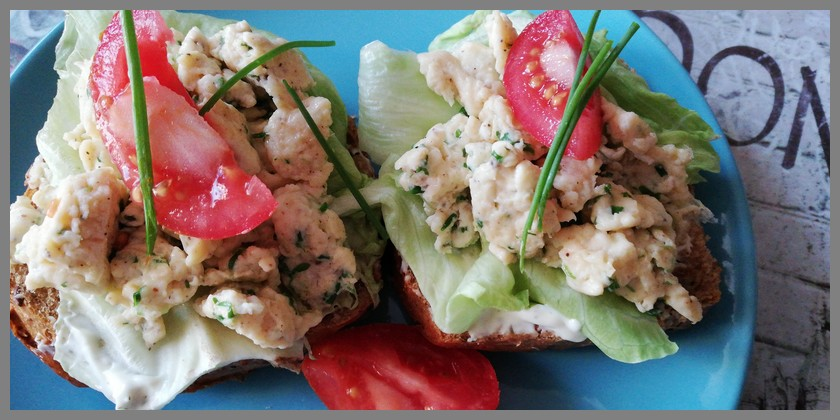
\includegraphics[width=\textwidth]{img/ruehrei_vollkorn.jpeg} \cite{ruehreivollkorn}

\subsection*{So geht's:}

\begin{tabular}{p{15cm}}
	\\
  Eier, Kräuter und Mineralwasser in einer Schüssel vermengen.\\
  Öl in einer flachen Pfanne erhitzen.\\
  Die Eimasse hineingeben, tocken lassen und nach und nach mit einem Schaber von außen nach innen schieben.\\
  In der Zwischenzeit die Brötchen aufschneiden und mit Remoulade bestreichen.\\
  Ein Salatblatt darauf platzieren.\\
  Das fertige Rührei auf dem Salat verteilen und mit einer halben Tomate garnieren.
\end{tabular}
